\documentclass[a4paper]{article}
\usepackage[spanish]{babel}
\usepackage[utf8]{inputenc}
\usepackage[usenames]{color}
\usepackage{charter}   % tipografia
\usepackage{graphicx}
\usepackage{enumerate}
\usepackage{listings}
\usepackage{color}
%\usepackage{indentfirst}
\usepackage{fancyhdr}
\usepackage{verbatim}
\usepackage{latexsym}
\usepackage{lastpage}
\usepackage[colorlinks=true, linkcolor=black]{hyperref}
%\usepackage{makeidx}
%\usepackage{float}
\usepackage{calc}
\usepackage{todonotes}
\usepackage{amsthm, amssymb}
\usepackage[nosumlimits]{amsmath} % este package hace que se vean mal los incides en las sumatorias, pero permite poner uno abajo del otro en la ecuacon de los L de laagrange

\usepackage{subfig}

\usepackage{amsfonts}
\definecolor{gray}{gray}{0.5}
\definecolor{light-gray}{gray}{0.95}
\definecolor{orange}{rgb}{1,0.5,0}

\usepackage{color} % para snipets de codigo coloreados
\usepackage{fancybox}  % para el sbox de los snipets de codigo

\definecolor{litegrey}{gray}{0.94}

% \newenvironment{sidebar}{%
% 	\begin{Sbox}\begin{minipage}{.85\textwidth}}%
% 	{\end{minipage}\end{Sbox}%
% 		\begin{center}\setlength{\fboxsep}{6pt}%
% 		\shadowbox{\TheSbox}\end{center}}
% \newenvironment{warning}{%
% 	\begin{Sbox}\begin{minipage}{.85\textwidth}\sffamily\lite\small\RaggedRight}%
% 	{\end{minipage}\end{Sbox}%
% 		\begin{center}\setlength{\fboxsep}{6pt}%
% 		\colorbox{litegrey}{\TheSbox}\end{center}}

\newenvironment{codesnippet}{%
	\begin{Sbox}\begin{minipage}{\textwidth}\sffamily\small}%
	{\end{minipage}\end{Sbox}%
		\begin{center}%
		\colorbox{litegrey}{\TheSbox}\end{center}}



\usepackage{fancyhdr}
\pagestyle{fancy}

%\renewcommand{\chaptermark}[1]{\markboth{#1}{}}
\renewcommand{\sectionmark}[1]{\markright{\thesection\ - #1}}

\fancyhf{}

\fancyhead[LO]{Sección \rightmark} % \thesection\ 
\fancyfoot[LO]{\small{Gustavo Cairo, Germán Pinzón, Ángel More}}
\fancyfoot[RO]{\thepage}
\renewcommand{\headrulewidth}{0.5pt}
\renewcommand{\footrulewidth}{0.5pt}
\setlength{\hoffset}{-0.8in}
\setlength{\textwidth}{16cm}
%\setlength{\hoffset}{-1.1cm}
%\setlength{\textwidth}{16cm}
\setlength{\headsep}{0.5cm}
\setlength{\textheight}{25cm}
\setlength{\voffset}{-0.7in}
\setlength{\headwidth}{\textwidth}
\setlength{\headheight}{13.1pt}

\renewcommand{\baselinestretch}{1.1}  % line spacing


\usepackage{underscore}
\usepackage{caratulaV}
\usepackage{url}
\usepackage{float}

\usepackage{underscore}
\usepackage{alltt}
\usepackage{tikz}
\usepackage{color}
\usepackage{verbatim}
\usepackage{algorithm}
\usepackage{algpseudocode}

\definecolor{dkgreen}{rgb}{0,0.6,0}
\definecolor{gray}{rgb}{0.5,0.5,0.5}
\definecolor{mauve}{rgb}{0.58,0,0.82}

\lstset{frame=tb,
  language=Python,
  aboveskip=3mm,
  belowskip=3mm,
  showstringspaces=false,
  columns=flexible,
  basicstyle={\small\ttfamily},
  keywordstyle=\color{blue},
  commentstyle=\color{dkgreen},
  stringstyle=\color{mauve},
  breaklines=true,
  breakatwhitespace=true,
  tabsize=3,
  numbers=left,
  xleftmargin=2em,
  frame=single,
  framexleftmargin=2em,
  numbersep=5pt,                   % how far the line-numbers are from the code
  numberstyle=\small\color{gray} % the style that is used for the line-numbers
 }

\parskip = 5 pt

\newcounter{row}
\newcounter{col}

\newcommand\setrow[3]{
	\setcounter{col}{1}
	\foreach \n in {#1, #2, #3} {
	\edef\x{\value{col} - 0.5}
	\edef\y{3.5 - \value{row}}
	\node[anchor=center] at (\x, \y) {\n};
	\stepcounter{col}
	}
	\stepcounter{row}
}



\newcommand\setrowaux[7]{
	\setcounter{col}{1}
	\foreach \n in {#1, #2, #3, #4, #5, #6, #7} {
	\edef\x{\value{col} - 0.5}
	\edef\y{7.5 - \value{row}}
	\node[anchor=center] at (\x, \y) {\n};
	\stepcounter{col}
	}
	\stepcounter{row}
}

\newcommand\setrowauxx[4]{
	\setcounter{col}{1}
	\foreach \n in {#1, #2, #3, #4} {
	\edef\x{\value{col} - 0.5}
	\edef\y{4.5 - \value{row}}
	\node[anchor=center] at (\x, \y) {\n};
	\stepcounter{col}
	}
	\stepcounter{row}
}


\begin{document}


\parskip = 5 pt
\thispagestyle{empty}
\materia{Aprendizaje Automático}
\titulo{Trabajo Práctico 1}
\integrante{Gustavo Cairo}{89/13}{gj.cairo@gmail.com}
\integrante{Germán Pinzón}{475/13}{pinzon.german.94@gmail.com}
\integrante{Ángel More}{931/12}{angel\_21\_fer@hotmail.com}

\maketitle

\newpage
\tableofcontents
\thispagestyle{empty}

\newpage
\section{Introducción}
El presente trabajo tiene como objetivo elaborar un clasificador de mails en Spam y Ham. Para lograr esto trabajaremos con distintos modelos de predicción.

Dado que los modelos necesitan de ciertos atributos para poder analizar, catalogar y así predecir , extraeremos un conjunto de atributos significativos de nuestro conjunto de mail.

Trabajaremos sobre un total de 90K de mails, de los cuales utilizaremos 70K como base de entrenamiento para los modelos y el resto como test set. 
 Evaluaremos distintas combinaciones y variaciones dentro de los modelos comparando la exactitud de cada uno así como el costo temporal que estos implican. 
 
 Finalmente seleccionaremos los mejores y los utilizaremos para clasificar a los mails perteneciente al test set y de esta manera tener una aproximación de como se comportaría el clasificador frente a nuevos datos.  
 
El código será elaborado en lenguaje python. Como bibliotecas destacadas utilizaremos $Pandas$, esta nos permitirá el almacenamiento de los mails y sus atributos dentro de la estructura $DataFrame$.

Las funciones que representen a los distintos modelos serán provistas por la biblioteca $sklearn$.

\subsection{Extracción de atributos}
Se realizaron un total de 505 extracciones de atributos sobre, aproximadamente, 70K de mails. Dicho conjunto de mails sera nuestro training set mientras que los 20K restantes se corresponderán con nuestro test set. Estos 20.000 mails de test fueron extraídos de manera aleatoria utilizando la función $random.sample$, y no fueron utilizados para el entrenamiento de los clasificadores.

Los atributos seleccionados fueron los siguientes:
\begin{itemize}
\item \textit{len}: longitud de cada mail.
\item \textit{count\_spaces}: cantidad de espacios que contienen los mails.
\item \textit{links}: cantidad de enlaces que contienen los mails. Lo consideramos importante ya que suponemos que un tipo de mail spam generalmente es aquel con publicidades y estos contienen distintos enlaces a sus diversos servicios comerciales; o así haciendo referencia a noticias.
\item \textit{tags}: cantidad de tags HTML encontrados. A veces podemos encontrar en los mails no sólo enlaces, sino imágenes, publicidades, noticias, etc. que se pueden visualizar dentro del propio mail, así como también formateo excesivo de los mismos (muchos colores, etc.) por lo que la presencia y/o cantidad de etiquetas HTML deberían constituir otro atributo distintivo.
\item \textit{rare}: este atributo representa la cantidad de caractere
\item 
s que podrían ser considerados poco comunes de encontrar en un mail del tipo Ham.
\item \textit{500 palabras que más aparecieron en los mails}: se extrajeron las 500 palabras más utilizadas del total de mails utilizados como base de entrenamiento. \\
Para la extracción se exceptuó tanto el encabezado de cada mail como la porción de texto que corresponde a mensajes reenviados. Tomamos estas decisiones porque de esta manera estamos excluyendo palabras que usualmente pueden estar presentes sin importar el tipo de mail, y por lo que considerarlas no nos brindaría ningún tipo información representativa a la hora de querer clasificarlos.     
\end{itemize}

\subsection{Modelos}
Decidimos trabajar con los siguientes algoritmos de aprendizaje:

\begin{itemize}
	\item Decision Tree Classifier
	\item Multinomial Naive Bayes Classifier
	\item Gaussian Naive Bayes Classifier
	\item KNN Classifier
	\item SVM Classifier
	\item Random Forest Classifier
\end{itemize}

Para todos los algoritmos que tuvieran hiperparámetros, elegimos un subset de los mismos (en base a nuestro conocimiento sobre ellos) y ejecutamos grid searches con varias alternativas de valores para cada uno. Ésto nos aseguró conseguir los mejores hiperparámetros (de entre los propuestos por nosotros) para cada clasificador. 
\newline

A continuación presentamos cuáles fueron los hiperparámetros seleccionados para cada algoritmo, y cuál fue su score correspondiente luego de ejecutar cross-validation de 10 folds con dichos parámetros.

\subsubsection{Decision Tree Classifier}
Para el Decision Tree Classifier variamos los siguientes hiperparámetros:
\begin{itemize}
	\item \textit{criterion:} el criterio para elegir qué atributo usar para hacer split.
	\item \textit{max\_features:} el número de atributos a tener en cuenta para buscar el mejor split.
	\item \textit{max\_depth:} la profundidad máxima del árbol (o sin límite).
	\item \textit{min\_samples\_split:} el mínimo número de instancias necesarias para subdividir un nodo.
\end{itemize}

\textit{Grid Search} arrojó que, entre todas las combinaciones propuestas, el mejor \textit{Decision Tree Classifier} era el que usaba \textit{entropy} como \textit{criterion}, tenía \textit{max\_features} igual a 10, \textit{max\_depth} sin límite, y \textit{min\_samples\_split} igual a 5. \newline
\indent El \textit{accuracy} arrojado luego de hacer cross-validation fue aproximadamente 0.96 ($+/-$0.012).

\subsubsection{Multinomial Naive Bayes Classifier}
Para el Multinomial Naive Bayes Classifier variamos los siguientes hiperparámetros:
\begin{itemize}
	\item \textit{alpha:} este parámetro modifica (\textit{suaviza}) la probabilidad de que un parámetro pertenezca a una clase.\footnote{Está relacionado a la frecuencia relativa. Más información: http://scikit-learn.org/stable/modules/naive_bayes.html\#multinomial-naive-bayes}
	\item \textit{fit\_prior:} este boolean determina si el algoritmo debería aprender la probabilidad de cada clase, o suponer una distribución uniforme.
\end{itemize}

\textit{Grid Search} arrojó que, entre todas las combinaciones propuestas, el mejor \textit{Multinomial Naive Bayes Classifier} era el que usaba \textit{fit\_prior} en \texttt{true}, y \textit{alpha} en 0.25. \newline
\indent El \textit{accuracy} arrojado luego de hacer cross-validation fue aproximadamente 0.65 ($+/-$0.06).

\subsubsection{Gaussian Naive Bayes Classifier}
El Gaussian Naive Bayes Classifier no toma parámetros, por lo que simplemente ejecutamos cross-validation. El \textit{accuracy} arrojado fue de 0.6 ($+/-$0.1).

\subsubsection{KNN Classifier}
Para el KNN Classifier variamos los siguientes hiperparámetros:
\begin{itemize}
	\item \textit{n_neighbors:} este parámetro define la cantidad de vecinos a usar.
	\item \textit{weights:} este parámetro define si los pesos dados a los vecinos son uniformes, o inversos a su distancia.
\end{itemize}

Hay un tercer parámetro con el cual intentamos experimentar, \textit{algorithm}, pero como utilizamos estructuras de datos esparsas para guardar el dataset y los atributos, el único algoritmo que funciona con estas estructuras (sin convertirlas en densas) es fuerza bruta. Al intentar utilizar algoritmos distintos, las máquinas en las cuales intentamos correr la Grid Search se quedaban sin memoria, así que optamos por utilizar simplemente el algoritmo de fuerza bruta.

\textit{Grid Search} arrojó que, entre todas las combinaciones propuestas, el mejor \textit{KNN Classifier} era el que usaba \textit{n\_neighbors} en 3, y \textit{weights} igual a \textit{distance}. \newline
\indent El \textit{accuracy} arrojado luego de hacer cross-validation fue aproximadamente 0.89 ($+/-$0.03).

\subsubsection{Gaussian Naive Bayes Classifier}
El Gaussian Naive Bayes Classifier no toma parámetros, por lo que simplemente ejecutamos cross-validation. El \textit{accuracy} arrojado fue de 0.6 ($+/-$0.1).

\subsubsection{SVM Classifier}
\todo{ESCRIBIR COSAS DE SVM}

\subsubsection{Random Forest Classifier}
Para el Random Forest Classifier variamos los siguientes hiperparámetros:
\begin{itemize}
	\item \textit{n_estimators:} este parámetro define la cantidad de árboles en el bosque.
	\item \textit{criterion:} el criterio para elegir qué atributo usar para hacer split.
	\item \textit{max\_features:} el número de atributos a tener en cuenta para buscar el mejor split.
	\item \textit{max\_depth:} la profundidad máxima del árbol (o sin límite).
	\item \textit{min\_samples\_split:} el mínimo número de instancias necesarias para subdividir un nodo.
\end{itemize}

\textit{Grid Search} arrojó que, entre todas las combinaciones propuestas, el mejor \textit{Random Forest Classifier} era el que usaba 20 árboles, \textit{criterion} igual a \textit{gini}, \textit{max\_features} igual a 1, \textit{max\_depth} igual a 2, y \textit{min\_samples\_split} también igual a 2. \newline
\indent El \textit{accuracy} arrojado luego de hacer cross-validation fue aproximadamente 0.98 ($+/-$0.006).

\subsection{Reducción de dimensionalidad}
Las técnicas que decidimos emplear para reducir la dimensionalidad fueron PCA, selección de $K$ mejores atributos y selección de percentil. Estas tres técnicas fueron combinadas siempre que fue posible y probadas con distintos parámetros en el caso de las últimas dos.

Para el caso de selección de $K$ mejores atributos variamos el K con los siguientes valores: 20, 50, 100, 150, 200, 250, 300, 320, 370, 400, 420 y 450 ya que pensamos que constituían una gama relativamente amplia de valores posibles, considerando que estamos trabajando con un total de 505 atributos. En el caso de la selección de percentil variamos el parámetro percentil con los valores 5, 10, 15 y 25. Además, dado que en algunos casos decidimos hacer una combinación de técnicas aplicando primero $PCA$ y luego alguna de las otras dos, también utilizamos dos funciones distintas en el parámetro $score\_func$ correspondiente a $SelectKBest$ y $SelectPercentile$.

Las funciones que utilizamos en el parámetro $score\_func$ fueron $chi2$ y $f\_classif$. Cuando decidimos aplicar primero $PCA$ y luego algún tipo de selección entonces tuvimos que utilizar la función $f\_classif$ debido a que si no se presentaban inconvenientes por valores negativos que aparecían en la matriz luego de la transformación que aplicaba $PCA$ ($chi2$ sólo acepta valores positivos, y PCA dejaba algunos valores negativos en el nuevo espacio). Sin embargo cuando aplicamos las funciones de selección por separado, sin combinarlas con $PCA$, pudimos experimentar tanto con $chi2$ como con $f\_classif$.

Un aspecto importante a rescatar es que tuvimos que hacer utilización de la clase $Pipeline$ de sklearn. Esto se debe a que como vamos a estar realizando ciertas transformaciones a los datos con los que nuestro clasificador vaya a entrenar, es necesario que dichas transformaciones se realicen en el momento indicado que es dentro de la función $cross\_val\_score$ (que usamos para medir la performance de nuestro clasificador en esta instancia). Así, si por ejemplo decidimos aplicar primero $PCA$ y luego $SelectKBest$ con $chi2$ y $K = 200$, entonces estas dos funciones (con parámetros en el caso de la segunda) van a ser steps en el pipeline que utilizará $cross\_val\_score$.

Finalmente para poder tener cierta variedad de transformaciones posibles en los datos a la hora de aplicar los clasificadores y decidir con cual quedarnos, vamos a estar aplicando lo siguiente:
\begin{itemize}
\item $PCA$
\item $SelectKBest$ con los valores de $K$ mencionados anteriormente y el parámetro $score\_func$ tanto con $f\_classif$ como con $chi2$
\item $SelectPercentile$ con los valores de $percentile$ mencionados anteriormente
\item $PCA$ y luego $SelectKBest$ (mismos valores de $K$ pero con $f\_classif$ en $score\_func$)
\item $PCA$ y luego $SelectPercentile$ (mismos valores de $percentile$)
\end{itemize}

Luego de hacer las transformaciones anteriores a los datos se aplicará cada uno de los clasificadores elegidos a excepción de Naive Bayes Multinomial en los casos donde se utilice $PCA$ ya que este clasificador no puede tratar ciertos valores negativos que aparecen en la matriz luego de la transformación.


\subsection{Resultados y selección del mejor clasificador}
Podemos describir nuestra estrategia para la elección del mejor clasificador de la siguiente forma:
\begin{itemize}
	\item  Luego de realizar Grid Search y buscar los mejores parámetros dentro de cierto rango para cada clasificador (a excepción de $SVM$ por su complejidad temporal y $GaussianNB$ porque no recibe parámetros), comparamos los valores de \textit{accuracy} arrojados por cross-validation (detallados en la sección de Modelos). En esta etapa ya es notorio que los clasificadores más performantes son Random Forest y Decision Tree, seguidos de KNN, y por último y con bastante peor desempeño, Naive Bayes Multinomial (se mostrarán los gráficos con los valores específicos más abajo).
	\item Por otro lado, como explicamos en la sección de reducción de dimensionalidad, también calculamos el score de cross-validation para cada clasificador sobre los datos transformados por cada una de las técnicas (o combinación de técnicas).
\end{itemize}

Una vez hecho lo anterior, procedimos a elegir la mejor configuración de datos que recibe cada clasificador. Es decir, en algunos casos una reducción de dimensionalidad pudo resultar más beneficiosa y en otros no, con lo cual para cada clasificador decidimos si vamos a transformar los datos antes de utilizarlo (y qué tipo de transformación vamos a estar realizando) o no. \\

Si bien más abajo se mostrarán los resultados de una manera gráfica y precisa, por lo general pudimos observar que aplicar alguna transformación a los datos siempre va a resultar mejor que no hacerlo. Una vez hecho esto, y seleccionados los clasificadores con sus correspondientes transformaciones, los aplicamos sobre los datos de test (que no fueron utilizados antes). Esto nos brinda una visión mucho más realista de la performance de nuestros clasificadores y nos da cierta seguridad de no haber estado haciendo \textit{overfitting} ya que, como mencionamos, estos datos fueron separados desde el principio y los clasificadores no fueron entrenados con ellos.



\begin{figure}[h]
    \centering
    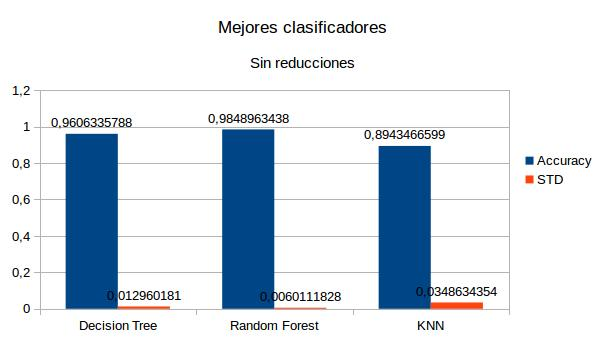
\includegraphics[width=0.75\textwidth]{imagenes/sinredtrain.jpg}
    \caption{Se muestran los clasificadores con un accuracy mayor a 0.8}
    \label{fig:1}
\end{figure}



\begin{figure}[h]
    \centering
    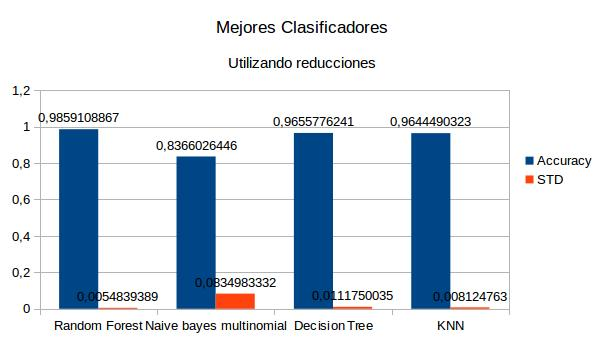
\includegraphics[width=0.75\textwidth]{imagenes/conredtrain.jpg}
    \caption{Se muestran los clasificadores con un accuracy mayor a 0.8 y las siguientes reducciones:\\
   Random Forest: 400 mejores atributos, usando chi2.\\
   Naive Bayes Multinomial: 200 mejores atributos, usando f\_classif.\\
   Decision tree: 200 mejores atributos, usando chi2.\\
   KNN: 50 mejores atributos, usando PCA y f_classif. }
    \label{fig:2}
\end{figure}
%
%\begin{figure}[h]
%    \centering
%    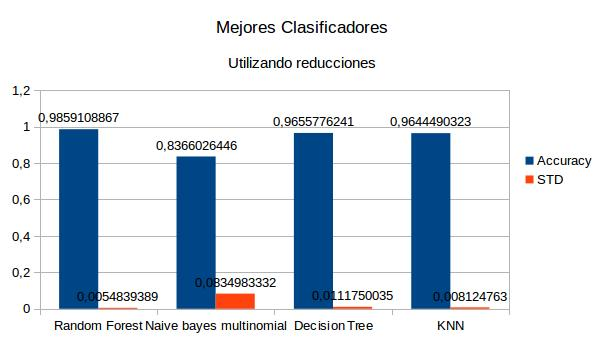
\includegraphics[width=0.75\textwidth]{imagenes/conredtrain.jpg}
%    \caption{Se muestran los clasificadores aplicados a la base de test, %con las reducciones de la \label{fig:2}}\\
%  \label{fig:2}
%\end{figure}

\subsection{Discusión}

  
A partir de las técnicas utilizadas y los distintos clasificadores utilizados hemos podido ver que los atributos seleccionados como los mejores generalmente variaban de un modelo a otro. Muchas veces esto ocurrió aun dentro de un mismo clasificador pero variando parámetros por ejemplo  $chi2$ o $f\_classif$. 

Aunque en nuestra selección de atributos predominan los del tipo 500 palabras mas usadas hemos visto que en algunos casos se ha tomado como los de mayor poder predictivo a los otros atributos. Con la reducción de dimensionalidad pudimos observar por un lado que los tiempos de ejecución de los distintos clasificadores disminuyeron respecto de sus versiones sin reducción. Además, observamos que en la mayoría de los casos al incrementar la cantidad de atributos el acurracy aumentaba pero cada vez de manera menos significativa. Incluso en algunos casos al aumentar el número de atributos el accuracy bajaba levemente de una iteración a otra.

 Esto nos llevo a buscar el mejor equilibrio entre las cantidad por un lado con pocos atributos tengo información escasa para poder distinguir entre un Spam y Ham pero, con demasiados atributos no solo aumenta el tiempo de computo sino que tener determinada combinación de atributos pueden empeorar la perfomance o caer en overfitting. 
 
Desde un primer momento observamos que Decision Tree y Random Forest fueron los que predominaron en todo momento la mayor exactitud se encontraba entre estos clasificadores. Aun así luego de observar todos los datos decidimos quedarnos con aquellos clasificadores que habían presentado una exactitud mayor al 80 \%, ya que por lo general estos clasificadores mantuvieron dicha calidad a lo largo de todas la experimentaciones. Una vez probados con la base de test este patrón vario un poco. En primer lugar la exactitud disminuyo mas de lo que habíamos pensado, lo cual puede ser causa de que, aun con las reducciones elegidas, estábamos  overfiteando. 
En segundo lugar los clasificadores que lideraron la exactitud no fueron los mismos que durante la experimentación....................

\section{Conclusión}

\end{document}